Tässä luvussa esitetään tutkimuksen tärkein sisältö ja kokonaisuutena vastaus tutkimuskysymykseen \emph{T1}, eli toistettavissa oleva menetelmä testitapauksien priorisoimiseen.
Priorisointiin vaikuttavat muuttujat luvussa \ref{ch:10_priorisointiin_vaikuttavat_muuttujat} esitetään myös suora vastaus tutkimuskysymykseen \emph{T2}.
Lisäksi painofunktiot \ref{ch:10_painofunktiot_priorisointiin} ja verkon karsiminen \ref{ch:10_verkon_karsiminen} esittää vastaukset tutkimuskysymykseen \emph{T3}.
Testitapauksien muodostaminen verkosta \ref{ch:10_testitapauksien_muodostaminen_verkosta} antaa osittaisen vastauksen myös tutkimuskysymykseen \emph{T4}.

Priorisointia varten esitetään harkintaa käyttäen valitut priorisointiin vaikuttavat muuttujat, niitä käyttävät painofunktiot, verkon rakentaminen ja karsiminen sekä verkon ja testitapauksien yhteys.
Lisäksi menetelmää käyttäen tuotetun painotetun verkon sisältämää informaatiota käytetään prioriteeteiltaan tärkeimmän polun löytämiseen.

\section{Priorisointiin vaikuttavat muuttujat} \label{ch:10_priorisointiin_vaikuttavat_muuttujat}

  Näkymä- ja siirtymäperustaiseen priorisointiin vaikuttavat monet eri asiat, joista osa kasvattaa prioriteettia ja osa laskee sitä.
  Prioriteettia kasvattava muuttuja on esimerkiksi liiketoiminnallinen arvo ja laskeva muuttuja on esimerkiksi projektin muutosherkkyys.
  Muuttujat ovat kuitenkin hyvin kontekstiriippuvaisia, joten yleispätevää ja kaikkiin tilanteisiin soveltuvaa listaa muuttujista on hankala antaa.
  Kontekstiriippuvaisuuden takia muuttujiin ja myöhemmin esitettäviin painofunktioihin on varattu paikka omille lisämuuttujille.

  Tässä diplomityössä esiteltävää priorisointimenetelmää varten jokainen priorisointiin vaikuttava muuttuja arvioidaan asteikolla 1-10, paria poikkeusta lukuun ottamatta.
  Numeerisella asteikolla on tarkoitus antaa korkea numero, jos muuttuja on prioriteetiltaan tärkeä kyseisen näkymän, eli verkon solmun kohdalla.
  Jos jokin muuttuja ei ole kelpoinen siinä kontekstissa, jossa menetelmää yritetään hyödyntää, tulee muuttujan arvo asettaa nollaksi, jolloin se sivuutetaan painofunktiossa \ref{ch:10_painofunktiot_priorisointiin}.

  Poikkeukselliset muuttujat ovat käyttötapauksien määrä ja siirtymien määrä, joissa numeerisen asteikon sijaan käytetään kyseisten muuttujien määrää suhteessa koko verkkoon.
  Esimerkiksi siirtymien määrää ilmaiseva suhde määritetään laskemalla solmun asteluku \(d_G(v)\), eli solmuun liittyneiden kaarien määrä, jaettuna kaikilla verkossa olevien kaarien määrällä.
  Lisäksi siirtymien määrän suhde vielä kerrotaan luvulla 10, jotta se saadaan skaalautumaan muiden muuttujien kanssa samalle tasolle.

  \begin{table}[H]
    \caption{Priorisointiin vaikuttavat muuttujat}
    \label{tab:priorisointiin_vaikuttavat_muuttujat}
    \centering
    \begin{tabular}{lllll} \hline
    \textbf{m} & \textbf{Muuttuja} & \textbf{Etumerkki} & \textbf{Asteikko} &  \\ \hline
    \textbf{1} & Liiketoiminnallinen arvo & + & 1 - 10 &  \\
    \textbf{2} & Liiketoiminnallinen visio & + & 1 - 10 &  \\
    \textbf{3} & Positiivinen käyttäjäpalaute & + & 1 - 10 &  \\
    \textbf{4} & Käyttötapauksien määrä & + & 10 \(\cdot\) suhde &  \\
    \textbf{5} & Siirtymien määrä & + & 10 \(\cdot\) suhde &  \\
    \textbf{6} & Negatiivinen käyttäjäpalaute & - & 1 - 10 &  \\
    \textbf{7} & Projektin muutosherkkyys & - & 1 - 10 &  \\
    \textbf{8} & Toteuttamisen kompleksisuus & - & 1 - 10 &  \\
    \textbf{9} & Toteutuksen virheherkkyys & - & 1 - 10 &  \\
    \textbf{10} & Omat lisämuuttujat & \(\pm\) & 1 - 10 &  \\ \hline
    \end{tabular}
  \end{table}

\section{Painofunktiot priorisointiin} \label{ch:10_painofunktiot_priorisointiin}

  Painofunktioiden määrittäminen on tärkeä osa painotetun verkon avulla priorisointia, sillä niiden avulla määritetään verkon solmujen ja kaarien prioriteetit.
  Tavanomaisesti numeerinen prioriteetti usein mielletään olevan korkea, jos priorisoitu muuttuja on tärkeä.
  Painotettujen verkkojen tapauksessa on kuitenkin järkevää vaihtaa numeerisen prioriteetin suuntaa, jotta painotettuun verkoon sovellettavat lyhimmän polun algoritmit toimisivat etsien prioriteetiltaan tärkeitä polkuja. Ennen prioriteetin suunnanvaihtoa, voidaan kokonaisprioriteetti \(p\) yksittäiselle solmulle \(v\), eli näkymälle määrittää seuraavasti.

  \[p(v) = \sum_{i=1}^{5} m_i - \sum_{j=6}^{9} m_j \pm m_{10}\]

  Prioriteetin suunnan vaihtamiseksi suuresta pieneen, säilyttäen kuitenkin prioriteetin sisältämän informaation, voi hoitaa käänteislukujen avulla.
  Ennen käänteisluvuksi muuttamista, prioriteettiin vaikuttavien muuttujien yhteenlaskettu summa voi olla ongelmallisesti negatiivinen tai nolla.
  Negatiiviset arvot eivät ole painotetun verkon kannalta erityisen järkeviä, sillä tässä diplomityössä hyödynnettävää Dijkstran algoritmia ei voida käyttää negatiivisien painojen kanssa.
  Dijkstran algoritmin toiminta nollan tapauksessa voi kuulostaa epäilyttävältä, kuten esimerkiksi tilanne, jossa painotetun verkon kaikki painot olisivat nollia.
  Dijkstran algoritmin tapauksessa tällainen verkko on kuitenkin sallittu, koska silloin lyhimmän polun ratkaisu on kaikki verkon solmut.
  Lyhimmän polun ongelman erityisvaatimusten lisäksi käänteislukua varten nolla on huono arvo siinä mielessä, että sille ei ole olemassa lainkaan käänteislukua.
  Nämä molemmat ongelmatapaukset voidaan painofunktiossa ratkaista siten, että käänteisfunktiota ei etsitä, vaan korvataan painofunktion tulos nollalla.

  Painofunktio yksittäiselle solmulle \(v\), eli näkymälle saadaan solmun kokonaisprioriteetin \(p(v)\) käänteislukuna.

  \[\alpha(v) = \begin{cases}
    p^{-1}(v) & p(v) > 0 \\
    0 & p(v) \leq 0
  \end{cases}\]

  Painofunktio yksittäiselle solmut \(v_1\) ja \(v_2\) yhdistävälle kaarelle \(e\), eli siirtymälle saadan myös käänteislukuna.
  Kaaren painofunktiota varten pitää kuitenkin huomioida, että sen kokonaisprioriteetti on kaaren solmujen kokonaisprioriteetin summa \(p(v_1) + p(v_2)\).
  Kaaren kokonaisprioriteetti \(p(v_1) + p(v_2)\) pitää laskea ennen käänteisluvuksi muuttamista.

  \[\beta(v) = \begin{cases}
    (p(v_1) + p(v_2))^{-1} & p(v_1) + p(v_2) > 0 \\
    0 & p(v_1) + p(v_2) \leq 0
  \end{cases}\]

\section{Verkon rakentaminen} \label{ch:10_verkon_rakentaminen}

  % TODO: Esitä esimerkkinäkymät ja relaatiot
  <TODO: Miten verkon solmut ja kaaret poimitaan käyttöliittymästä>

  <TODO: Selitä A-J näkymät, jota varten painomatriisi ja esimerkkigraafi on tehty.
  \begin{itemize}
    \item \textbf{A:} Kirjautumisnäkymä
    \item \textbf{B:} Pelivalikkonäkymä
    \item \textbf{C:} Pelinäkymä
    \item \textbf{D:} Asetusnäkymä
    \item \textbf{E:} Ostonäkymä
    \item \textbf{F:} Ohjenäkymä
    \item \textbf{G:} Tulosnäkymä
    \item \textbf{H:} Onnittelunäkymä
  \end{itemize}

  % TODO: Päivitä painomatriisi vastaamaan esimerkkiä
  <TODO: Esimerkki painomatriisista, jota käytetään priorisoinnin syötteenä>
  \[
    M_G =
    \bordermatrix{
      G & v_a & v_b & v_c & v_d & v_e & v_f & v_g & v_h & v_i & v_j \cr
      v_a & \infty & 1 & 1 & 1 & 1 & 1 & 1 & 1 & 1 & 1 \cr
      v_b & 1 & \infty & 1 & 1 & 1 & 1 & 1 & 1 & 1 & 1 \cr
      v_c & 1 & 1 & \infty & 1 & 1 & 1 & 1 & 1 & 1 & 1 \cr
      v_d & 1 & 1 & 1 & \infty & 1 & 1 & 1 & 1 & 1 & 1 \cr
      v_e & 1 & 1 & 1 & 1 & \infty & 1 & 1 & 1 & 1 & 1 \cr
      v_f & 1 & 1 & 1 & 1 & 1 & \infty & 1 & 1 & 1 & 1 \cr
      v_g & 1 & 1 & 1 & 1 & 1 & 1 & \infty & 1 & 1 & 1 \cr
      v_h & 1 & 1 & 1 & 1 & 1 & 1 & 1 & \infty & 1 & 1 \cr
      v_i & 1 & 1 & 1 & 1 & 1 & 1 & 1 & 1 & \infty & 1 \cr
      v_j & 1 & 1 & 1 & 1 & 1 & 1 & 1 & 1 & 1 & \infty \cr
    }
  \]

  % TODO: Päivitä kuva vastaamaan esimerkkiä
  <TODO: Esimerkki painotetusta verkosta, jota käytetään priorisoinnin syötteenä>
  \begin{figure}[H]
    \centering
    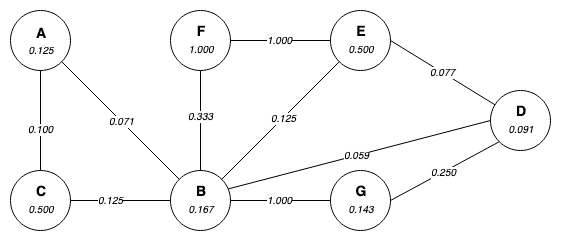
\includegraphics[width=0.8\textwidth]{assets/painotettu-verkko-ennen.png}
    \caption{Esimerkki painotetusta verkosta ennen leikkauksia}
    \label{fig:painotettu-verkko-ennen}
  \end{figure}

\section{Verkon karsiminen} \label{ch:10_verkon_karsiminen}

  Painotetun verkon karsiminen eli leikkaaminen on prioriteeillä painotetun verkon tärkeä ominaisuus.
  Verkkoteorian soveltaminen prioriteettien avulla painotettuun verkkoon on erityisen hyödyllistä, kun verkon kaarissa korkea paino tarkoittaa suurta prioriteettia.
  Tällaisessa tapauksessa on mahdollista soveltaa lyhimmän polun ongelman ratkaisemiseen kehitettyjä algoritmeja, jolloin ne toimivat etsien alhaisimman prioriteetin polkuja.
  Lyhimmän polun etsimiseen on tarkoituksenmukaista valita aina aloitus ja lopetuspisteet, joiden välille lyhin polku verkossa voidaan etsiä.
  Prioriteetein painotetun verkon karsimistarkoitukseen olisi järkevää valita sellaiset aloitus- ja lopetuspisteet, joiden välillä ei näyttäisi olevan korkean prioriteetin solmuja.
  Voidaan kuitenkin menetellä myös siten, että valitaan aloitus- ja lopetuspisteeksi sellaiset solmut, jotka ovat painoltaan verkon alhaisimmat \(v_1 = min(V)\) ja \(v_2 = min(V \setminus \{v_1\})\) ja esimerkiksi verrata niiden lyhimmän polun kokonaisprioriteettia muuhun verkkoon.

  \begin{itemize}
    \item Pienimmän prioriteetin solmuparin etsiminen, eli \(v_1 = min\{ \alpha(V) \}\) ja \(v_2 = min\{\alpha( V \setminus \{v_1\} \}\).
    \item Dijkstran algoritmin käyttö lyhimmän (prioriteetiltaan pienimmän) polun löytämiseen, eli \(s = min( \gamma(P) ), P \in G\).
    \item Leikkauksien tekeminen ja toistaminen \(n\)-kertaa.
    \item Poistetaan yhden yksittäiseen solmuun johtavat sillat, jossa \(\alpha(v) < aivan liian alhainen \).
    \item Poistetaan kaikki yksittäiset eristetyt solmut, eli asteluku on nolla \(d_G(X) = 0\).
    \item Poistetaan Dijkstran lyhimmän polun kaaret, jossa \(\beta(e) < liian alhainen \).
  \end{itemize}

  % TODO: Päivitä kuva vastaamaan esimerkkiä
  \begin{figure}[H]
    \centering
    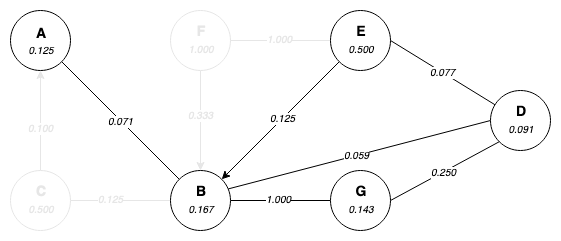
\includegraphics[width=0.8\textwidth]{assets/painotettu-verkko-jalkeen.png}
    \caption{Esimerkki painotetusta verkosta leikkauksien jälkeen}
    \label{fig:painotettu-verkko-jalkeen}
  \end{figure}

\section{Dijkstran algoritmin hyödyntäminen} \label{ch:10_dijkstran_algoritmin_hyodyntaminen}

  <TODO: Valitaan min v1 ja v2 ja käytetään dijkstran algoritmia niille>

\section{Verkon ja testitapauksien yhteys} \label{ch:10_verkon_ja_testitapauksien_yhteys}

  Ennen testitapauksien suunnittelua tehtävä priorisointi kuvainnollistaa käyttöliittymän näkymiä, niiden osanäkymiä ja niiden välisiä siirtymiä.
  Tällaisesta painotetusta verkosta saadaan priorisoitua näkymät ja siirtymät, mutta lopulliset testitapauksien prioriteetit ovat testitapaukseen kuuluvien näkymien tai siirtymien prioriteetteja.
  Tämä tarkoittaa käytännössä sitä, että kun näkymät ja siirtymät on priorisoitu, on esimerkiksi yhden yksittäisen tarkasteltavana olevan näkymän toiminnoilla sama keskenään prioriteetti.
